\documentclass[]{kling/kling}
%\usepackage[table,dvipsnames]{xcolor}
% Option "twocolumn" available, but please prioritize single-column

\usepackage{microtype}
\usepackage{graphicx}
\usepackage{subcaption}
%\usepackage{booktabs} % for professional tables
\usepackage{csquotes}
\usepackage{afterpage}

% For theorems and such
\usepackage{amsmath}
\usepackage{amssymb}
\usepackage{mathtools}
\usepackage{amsthm}
\usepackage{xspace}
\usepackage{colortbl}
\usepackage{multirow}
\usepackage{enumitem}
\usepackage{wrapfig}
\usepackage{nicefrac}

%%%% method abbreviations %%%%
\newcommand{\putalg}{{\small V-JEPA}\xspace}
\newcommand{\model}{V-JEPA~2\xspace}
\newcommand{\oldModel}{V-JEPA\xspace}
\newcommand{\acModel}{V-JEPA~2-AC\xspace}
%%%% end of method abbreviations %%%%

\newcommand{\cc}{\cellcolor{klingbg}}
\newcommand{\ccg}{\cellcolor{klingbg}}
\newcommand{\fcg}{\color{black}}

\newcommand\todo[1]{\textcolor{red}{#1}}

%%% tile and authors %%%
\title{V-JEPA~2: Self-Supervised Video Models Enable Understanding, Prediction and Planning}
\headertext{V-JEPA 2: Self-Supervised Video Models}

\author[1*]{Mahmoud Assran}
\author[1\dag]{Adrien Bardes}
\author[1]{David Fan}
\author[1]{Quentin Garrido}
\author[1]{Russell Howes}
\author[1]{Mojtaba Komeili}
\author[1]{Matthew Muckley}
\author[1]{Ammar Rizvi}
\author[1]{Claire Roberts}
\author[1]{Koustuv Sinha}
\author[1,2]{Artem Zholus}
\author[1]{Sergio Arnaud}
\author[1]{Abha Gejji}
\author[1]{Ada Martin}
\author[1\dag]{Francois Robert Hogan}

\affiliation[1]{FAIR at Meta}
\affiliation[2]{Mila -- Quebec AI Institute and Polytechnique Montr\'{e}al}

%%% footnotes %%%
\renewcommand{\thefootnote}{\fnsymbol{footnote}}
\footnotetext[1]{Work done during an internship at Kling Team, Kuaishou Technology.}
\footnotetext[2]{Corresponding authors.}

%%% abstract %%%
\abstract{
A major challenge for modern AI is to learn to understand the world and learn to act largely by observation~\citep{lecun2022path}.
This paper explores a self-supervised approach that combines internet-scale video data with a small amount of interaction data (robot trajectories), to develop models capable of understanding, predicting, and planning in the physical world. We first pre-train an action-free joint-embedding-predictive architecture, \model, on a video and image dataset comprising over 1 million hours of internet video. \model achieves strong performance on motion understanding (77.3 top-1 accuracy on Something-Something v2) and state-of-the-art performance on human action anticipation (39.7 recall-at-5 on Epic-Kitchens-100) surpassing previous task-specific models. Additionally, after aligning \model with a large language model, we demonstrate state-of-the-art performance on multiple video question-answering tasks at the 8 billion parameter scale (e.g., 84.0 on PerceptionTest, 76.9 on TempCompass). Finally, we show how self-supervised learning can be applied to robotic planning tasks by post-training a latent action-conditioned world model, \acModel, using less than 62 hours of unlabeled robot videos from the Droid dataset. We deploy \acModel zero-shot on Franka arms in two different labs and enable picking and placing of objects using planning with image goals. Notably, this is achieved without collecting any data from the robots in these environments, and without any task-specific training or reward. This work demonstrates how self-supervised learning from web-scale data and a small amount of robot interaction data can yield a world model capable of planning in the physical world.
}

% additional metadata %%%
\metadata[Data]{June 13, 2025}
\metadata[Correspondence]{Nicolas Ballas <ballasn@meta.com> and Michael Rabbat <mikerabbat@meta.com>}
\metadata[Code]{\url{https://github.com/facebookresearch/vjepa2}}
\metadata[Blogpost]{\url{https://ai.meta.com/blog/v-jepa-2-world-model-benchmarks}}
\metadata[Project Page]{\url{ https://ai.facebook.com/vjepa2/}}

\begin{document}

\maketitle

\section{Introduction}
\label{section:intro}

Humans have the ability to adapt and generalize when taking on new tasks and operating in unfamiliar environments.
Several cognitive learning theories suggest that humans learn an internal model of the world by integrating low-level sensory inputs to represent and predict future states~\citep{craik1967nature,rao1999predictive}, and they further posit that this world model shapes our perception at any given moment, playing a crucial role in informing our understanding of reality~\citep{friston2010free,clark2013whatever,nortmann2015primary}.
Moreover, our ability to predict the effects of our actions on future states of the world is also essential for goal-oriented planning~\citep{sutton1981adaptive,sutton1998reinforcement,ha2018world,wolpert2000computational}.
Building artificial agents that learn a world model from sensory data, such as video, could enable them to \emph{understand} the physical world, \emph{predict} future states, and effectively --- like humans --- \emph{plan} in new situations, resulting in systems capable of tackling tasks that have not been encountered before.

\begin{figure}[!t]
    \centering
    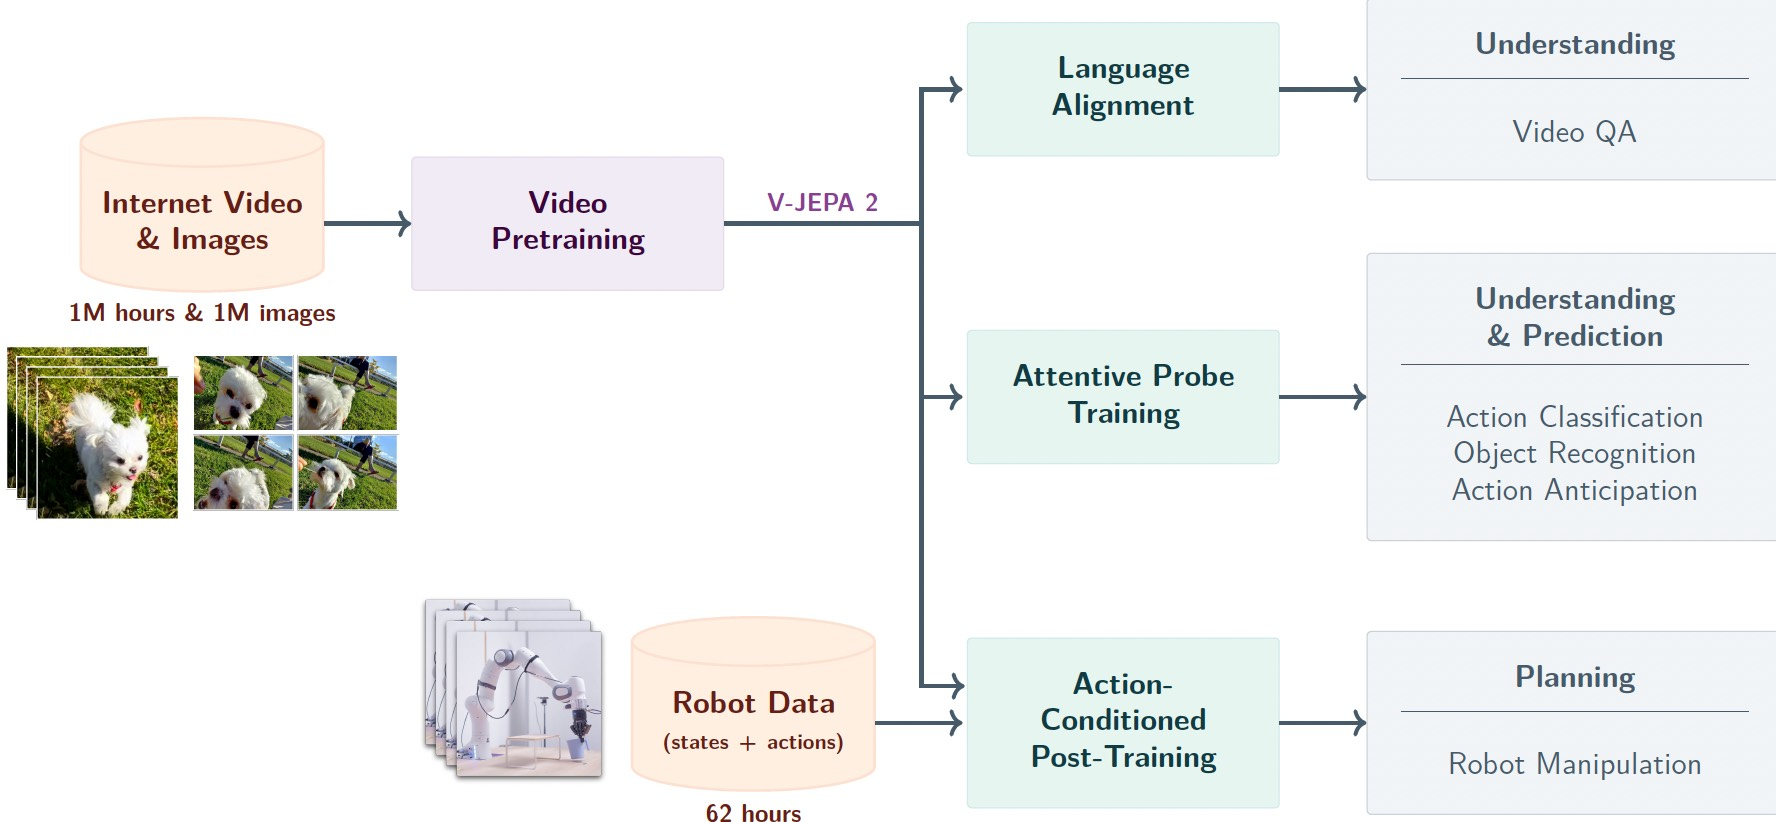
\includegraphics[width=\linewidth]{assets/flowchart.jpg}
    \caption{{\bf \model Overview.}
    Leveraging 1M hours of internet-scale video and 1M images, we pretrain the \model video model using a visual mask denoising objective~\citep{bardes2024revisiting, assran2023self}, and leverage this model for downstream tasks such as action classification, object recognition, action anticipation, and Video Question Answering by aligning the model with an LLM backbone.
    After pretraining, we can also freeze the video encoder and train a new action-conditioned predictor with a small amount of robot interaction data on top of the learned representations, and leverage this action-conditioned model, \acModel, for downstream robot manipulation tasks using planning within a model predictive control loop.}
    \label{fig:overview}
\end{figure}

Previous works have explored the development of predictive world models from interaction data consisting of state-action sequences, often also relying on explicit reward feedback from the environment to infer goals~\citep{sutton1981adaptive,fragkiadaki2015learning,ha2018world,hafner2019learning,hansen2022temporal}. However, the limited availability of real-world interaction data constrains the scalability of these methods.
To address this limitation, more recent works have leveraged both internet-scale video and interaction data towards training action-conditioned video generation models for robot control, but only demonstrate limited results in robot execution using model-based control~\citep{hu2023gaia,yang2024learning,bruce2024genie,agarwal2025cosmos}.
In particular, this line of research often emphasizes the evaluation of the faithfulness of the predictions and visual quality instead of planning capabilities, perhaps due to the computational cost of planning by generating video.

In this work, we build upon the self-supervised hypothesis as a means to learn world models that capture background knowledge of the world largely from observation. Specifically, we leverage the joint-embedding predictive architecture (JEPA)~\citep{lecun2022path}, which learns by making predictions in a learned representation space.
In contrast to approaches that focus on learning entirely from interaction data, self-supervised learning enables us to make use of internet-scale video --- depicting sequences of states without direct observations of the actions ---
to learn to both represent video observations and learn a predictive model for world dynamics in this learned representation space.
Furthermore, in contrast to approaches based on video generation, the JEPA approach focuses on learning representations for predictable aspects of a scene (e.g., the trajectory of an object in motion) while ignoring unpredictable details that generative objectives emphasize, since they make pixel-level predictions (e.g., the precise location of each blade of grass in a field, or each leaf on a tree).
By scaling JEPA pretraining, we demonstrate that it yields video representations with state-of-the-art understanding and prediction capabilities, and that such representations can be leveraged as a basis for action-conditioned predictive models and enable zero-shot planning.

Our approach, \model, utilizes a stage-wise training procedure, beginning with action-free pre-training on internet-scale video, followed by post-training with a small amount of interaction data (see \Cref{fig:overview}).
In the first stage, we use a mask-denoising feature prediction objective~\citep{assran2023self,bardes2024revisiting}, where the model predicts masked segments of a video in a learned representation space.
We train the \model  encoder with up to 1 billion parameters and with more than 1 million hours of video.
Our experiments confirm that scaling self-supervised  video pretraining enhances the encoder's ability to achieve visual understanding, including broad motion and appearance recognition capabilities, through probe-based evaluations and by aligning the encoder with a language model for video question-answering \citep{benno2024, patraucean2023perception, liu2024tempcompass, cai2024temporalbench, shangguan2024tomato}.


Following pretraining on internet-scale video, we train an action-conditioned world model, \acModel, on a small set of interaction data using the representations learned in the first stage.
Our action-conditioned world model is a 300M-parameter transformer network employing a block-causal attention mechanism, which autoregressively predicts the representation of the next video frame conditioned on an action and previous states.
With as little as 62 hours of unlabeled interaction data from the Droid dataset~\citep{khazatsky2024droid}, we demonstrate the feasibility of training a latent world model that, given sub-goals, can be leveraged to plan actions on a Franka robot arm and perform prehensile manipulation tasks from a monocular RGB camera zero-shot in a new environment.

To summarize, we show that joint-embedding predictive architectures learning from videos can be used to build a world model that enables \emph{understanding} the physical world, \emph{predicting} future states, and effectively \emph{planning} in new situations; this is achieved by leveraging internet-scale video and a small amount of interaction data.
Specifically:
\begin{itemize}


\item \textit{Understanding --- Probe-based Classification:} Scaling self-supervised video pretraining results in video representations applicable to many tasks. \model excels at encoding fine-grained motion information, achieving strong performance on tasks requiring motion understanding, such as Something-Something~v2, with $77.3$ top-1 accuracy using an attentive probe.


\item \textit{Understanding --- Video Question-Answering:} \model encoder can be used to train a multi-modal large language model, to tackle video-question answering tasks. We observe state-of-the-art performance on 8B language model class on multiple benchmarks that require physical world understanding and temporal reasoning, such as MVP ($44.5$ paired accuracy), PerceptionTest ($84.0$ test set accuracy), TempCompass ($76.9$ multi-choice accuracy), TemporalBench ($36.7$ multi-binary short-QA accuracy) and TOMATO ($40.3$ accuracy).  In particular, we show that a video encoder pre-trained \textit{without} language supervision can be aligned with a language model and achieve state-of-the-art performance, contrary to conventional wisdom~\citep{yuan2025tarsier2, wang2024internvideo2}.

\item \textit{Prediction:} Large-scale self-supervised video pretraining enhances prediction capabilities.  \model achieves state-of-the-art performance on the Epic-Kitchens-100 human-action anticipation task using an attentive probe, with $39.7$ recall-at-5, which is a $44$\% relative improvement over the previous best model.

\item \textit{Planning:} We demonstrate that \acModel, obtained by post-training \model with only $62$ hours of unlabeled robot manipulation data from the popular Droid dataset, can be deployed in new environments to solve prehensile manipulation tasks using planning with given subgoals.
Without training on any additional data from robots in our labs, and without any task-specific training or reward, the model successfully handles prehensile manipulation tasks, such as Grasp and Pick-and-Place with novel objects and in new environments.
\end{itemize}

The remainder of this paper is organized as follows.
\Cref{section:stage1} describes the \model pretraining procedure, including the key ingredients enabling scaling beyond the original V-JEPA recipe of \citet{bardes2024revisiting}.
\Cref{section:stage2} then introduces our approach to training a task-agnostic action-conditioned world model, \acModel, leveraging the pretrained \model model.
\Cref{sec:robot_planning} demonstrates using \acModel for robot control via model-based planning.
Because \acModel models world dynamics in a learned representation space, its capabilities fundamentally depend on the information captured in the \model representation space, and so we further explore the performance of \model for video understanding in \Cref{sec:encoder_comparison} and prediction tasks in \Cref{section:prediction}.
Finally, in \Cref{section:language_understanding} we show that \model can be aligned with a language model for video question answering.
\Cref{section:related_work} discusses related work, and we conclude in \Cref{section:conclusion}.

\begin{figure}[!t]
    \centering
    \begin{subfigure}[T]{0.33\textwidth}
        \centering
        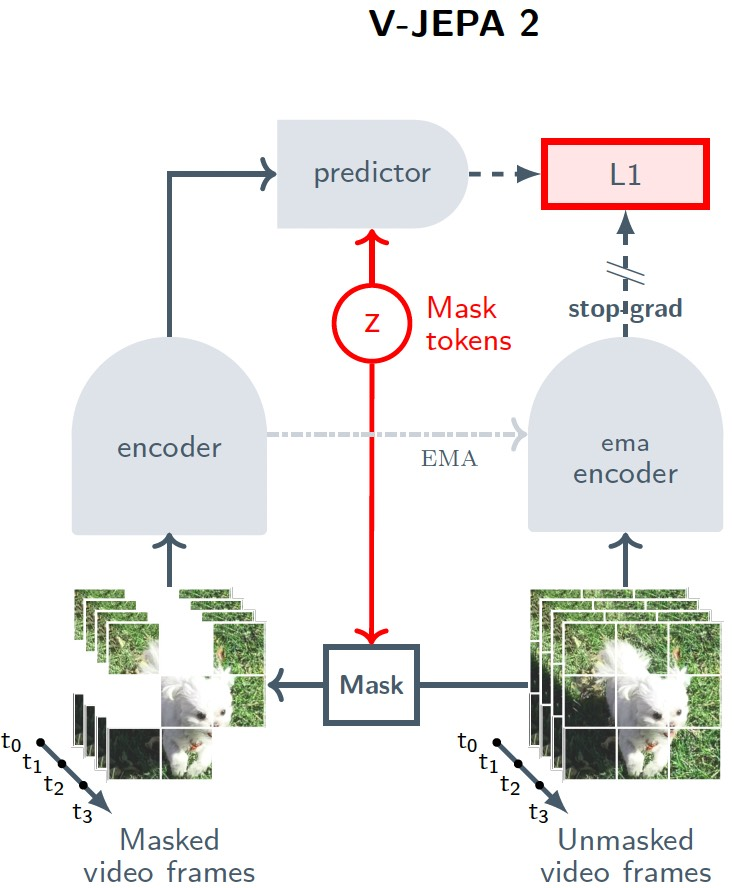
\includegraphics[width=\linewidth]{assets/vjepa2-abstract-new.jpg}
    \end{subfigure}
    \quad\quad\quad {\color{gray}\vrule} \quad\quad\quad
    \begin{subfigure}[T]{0.33\textwidth}
        \centering
        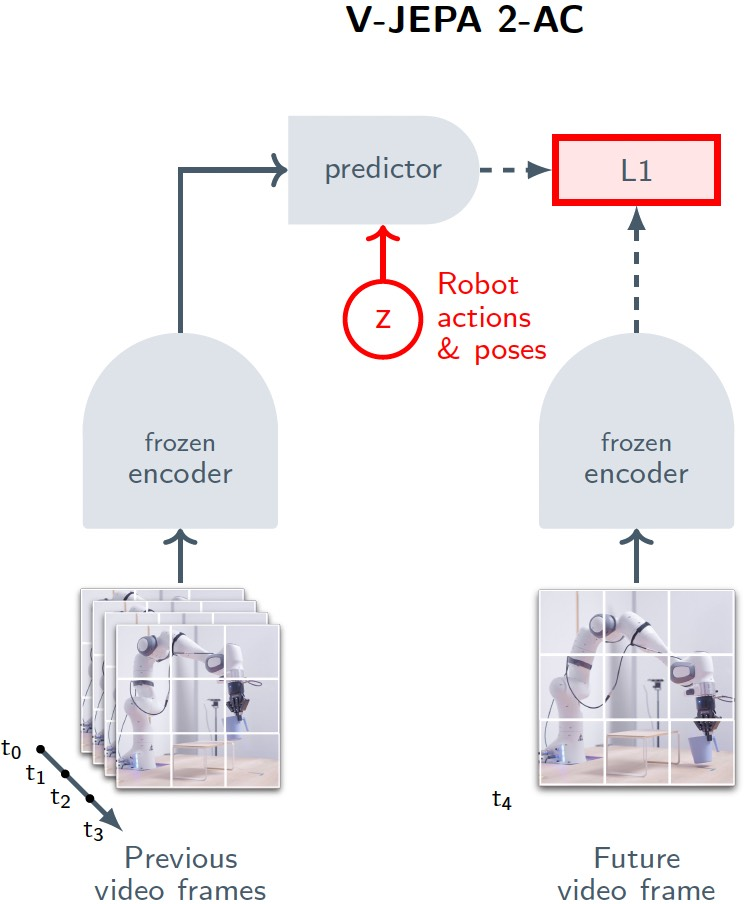
\includegraphics[width=\linewidth]{assets/vjepa2-ac-abstract-new.jpg}
    \end{subfigure}
    \hfill
    \caption{{\bf Multistage training.}
    {\bf (Left)} We first pretrain the \model video encoder on internet-scale image and video data using a visual mask denoising objective~\citep{bardes2024revisiting, assran2023self}.
    A video clip is patchified into a sequence of tokens and a mask is applied by dropping a subset of the tokens.
    The encoder then processes the masked video sequence and outputs an embedding vector for each input token.
    Next, the outputs of the encoder are concatenated with a set of learnable mask tokens that specify the position of the masked patches, and subsequently processed by the predictor.
    The outputs of the predictor are then regressed to the prediction targets using an L1 loss.
    The prediction targets are computed by an ema-encoder, the weights of which are defined as an exponential moving average of the encoder weights.
    {\bf (Right)} After pretraining, we freeze the video encoder and learn a new action-conditioned predictor, \acModel, on top of the learned representation.
    We leverage an autoregressive feature prediction objective that involves predicting the representations of future video frames conditioned on past video frames, actions, and end-effector states.
    Our action-conditioned predictor uses a block-causal attention pattern such that each patch feature at a given time step can attend to the patch features, actions, and end-effector states from current and previous time steps.
    }
    \label{fig:multistage_training}
\end{figure}


\section{V-JEPA~2: Scaling Self-Supervised Video Pretraining}
\label{section:stage1}

We pretrain \model on a visual dataset that includes over 1 million hours of video. The self-supervised training task is based on mask denoising in representation space and builds upon the V-JEPA framework~\citep{bardes2024revisiting}. In this paper, we extend the V-JEPA framework by exploring larger-scale models, increasing the size of the pretraining data, and introducing a spatial and temporal progressive resolution training strategy that enables us to efficiently pretrain models beyond short 16-frame video clips.


\subsection{Methodology}

\paragraph{\bf Mask-Denoising in Representation Space.}
The V-JEPA objective aims to predict the learned representation of a video $y$ from a view $x$ of that video that has been masked, i.e., from which patches have been randomly dropped (\Cref{fig:multistage_training}, left). The task meta-architecture consists of an encoder, $E_\theta(\cdot)$, which extracts video representations, and a predictor, $P_\phi(\cdot)$, which predicts the representation of masked video parts. The encoder and predictor are trained simultaneously using the objective,
\begin{equation}
\label{eq:loss}
\text{minimize}_{\theta,\phi, \Delta_y}\quad \lVert P_\phi(\Delta_y, E_\theta(x)) - \text{sg}(E_{\overline\theta}(y)) \rVert_1,
\end{equation}
where $\Delta_y$ is a learnable mask token that indicates the locations of the dropped patches. The loss uses a stop-gradient operation, $\text{sg}(\cdot)$, and an exponential moving average, $\overline \theta$, of the weights $\theta$ of the encoder network to prevent representation collapse. The loss is applied only to the predictions of the masked patches.

\paragraph{\bf Architecture.} The encoder, $E_\theta(\cdot)$, and predictor, $P_\phi(\cdot)$, are each parameterized as a vision transformer~\citep{dosovitskiy2020image} (or ViT).
To encode relative position information in the vision transformer, we leverage RoPE (Rotary Position Embedding) instead of the absolute sincos position embedding used in~\citet{bardes2024revisiting}. We use a 3D extension of traditional 1D-RoPE~\citep{su2024roformer} by partitioning the feature dimension into three approximately equal segments (for the temporal, height, and width axes) and applying the 1D rotations separately to the segment for each axis.
We found that using 3D-RoPE instead of absolute sincos position embeddings~\citep{vaswani2017attention} helps stabilize training for the largest models.
To process a video with our transformer encoder, we first patchify it as a sequence of tubelets of size $2\times16\times16$ ($T\times H\times W$) and employ the same multiblock masking strategy as in~\citet{bardes2024revisiting}.

\paragraph{\bf Key Scaling Ingredients.} In this section we introduce and study four additional key ingredients which enable scaling the V-JEPA pre-training principle to obtain our \model model.
\begin{enumerate}
\item \emph{Data scaling:} We increase the dataset size from 2~million to 22~million videos by leveraging and curating additional data sources.

\item \emph{Model scaling:} We scale the encoder architecture from 300~million to over 1~billion parameters, going from a ViT-L to a ViT-g \citep{zhai2022scaling}.

\item \emph{Longer training:} Adopting a warmup-constant-decay learning rate schedule simplifies hyperparameter tuning and enables us to extend training from 90~thousand up to 252~thousand iterations, effectively leveraging the additional data.

\item \emph{Higher resolution:} We leverage the warmup-constant-decay schedule to efficiently scale to higher resolution video and longer video clips by training on shorter, lower-resolution clips during the warmup and constant phases, and then increasing resolution and/or clip-length during the final decay phase.
\end{enumerate}
The remainder of this section describes each of these ingredients in further detail and also quantifies the impact of each ingredient using the evaluation protocol described next.

\begin{wrapfigure}{r}{0.4\textwidth}
    \centering
    \small
    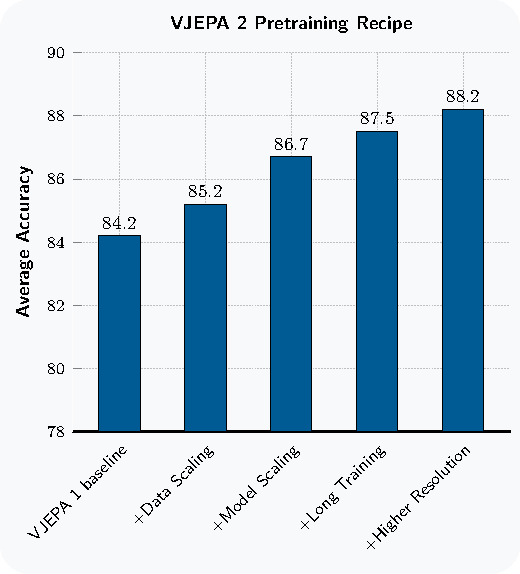
\includegraphics[width=\linewidth]{assets/v1_to_v2.pdf}
    \caption{{\bf Scaling Ingredients.}
    The effects of scaling interventions on average accuracy across 6 image and video classification tasks (SSv2, Diving-48, Jester, Kinetics, COIN, ImageNet) using a ViT-L/16 model as baseline.
    }
    \label{fig:v1_to_v2}
    \vspace{-2em}
\end{wrapfigure}
\paragraph{\bf Evaluation Protocol.} Our goal with model pretraining is to infuse general visual understanding into our encoder. We therefore evaluate our model and data design choices by assessing the quality of the model's learned representation on a set of six motion and appearance classification tasks: Something-Something v2~\citep{goyal2017something}, Diving-48~\citep{li2018resound},  Jester~\citep{materzynska2019jester}, Kinetics~\citep{kay2017kinetics}, COIN~\citep{tang2019coin}, and ImageNet~\citep{deng2009imagenet}. We use a frozen evaluation protocol: we freeze the encoder weights and train a task-specific 4-layers attentive probe on its representation to output a predicted class. In this section, we focus mainly on the average accuracy across the six understanding tasks. Refer to~\Cref{sec:encoder_comparison} for additional details about the tasks, evaluation protocol, and results.
\subsection{Scaling Self-Supervised Video Learning}

We first present a summary of the key findings of our scaling analysis, where we investigate the impact of the four key ingredients on downstream task average performance.
\Cref{fig:v1_to_v2} illustrates the effects of these scaling interventions on average accuracy across 6 classification tasks, using a ViT-L/16 model pretrained on 2 million videos with the V-JEPA objective as our baseline.
Increasing the dataset from 2 million to 22 million videos (VM22M) yields a 1.0-point improvement. Scaling the model from 300 million to 1 billion parameters (ViT-g/16) provides an additional 1.5-point gain. Extending training from 90K to 252K iterations contributes another 0.8-point improvement. Finally, enhancing both spatial resolution ($256\time256 \rightarrow 384\time384$) and temporal duration  ($16 \rightarrow 64$ frames), during both pretraining and evaluation,  boosts performance to 88.2\%, representing a cumulative 4.0-point improvement over the ViT-L/16 baseline. Each individual change provides a positive impact, confirming the potential of scaling in video self-supervised learning (SSL).



\subsection{Pretraining Dataset}
\label{subsec:pretraining_dataset}

Next, we describe the sources of videos and images that make up our pretraining dataset, and our approach to curating the dataset.
\begin{table}[t!]
    \centering
    \small
    \caption{
      \textbf{VideoMix22M (VM22M) Pretraining Dataset.}
      To build our observation pretraining dataset, we combined four different video sources and one image dataset. We use a source-specific sampling probability during training and apply retrieval-based curation on YT1B to reduce noisy content (e.g., cartoon- or clipart-style).}
    \begin{tabular}{ccccccc}
    \toprule
    Source & Samples & Type & Total Hours &  Apply Curation  & Weight\\
    \midrule
    SSv2~\citep{goyal2017something} & 168K & EgoVideo  & 168 & No & 0.056\\
    Kinetics~\citep{carreira2019short} & 733K & ExoVideo  & 614 & No & 0.188\\
    Howto100M~\citep{miech2019howto100m} & 1.1M & ExoVideo  & 134K & No & 0.318\\
    YT-Temporal-1B~\citep{zellers2022merlot} & 19M & ExoVideo  & 1.6M & Yes & 0.188\\
    ImageNet~\citep{deng2009imagenet} & 1M & Images  & n/a & No & 0.250\\
    \end{tabular}
    \label{table:pretraining_dataset}
\end{table}

\paragraph{\bf Scaling Dataset Size.}
We construct a large-scale video dataset by combining publicly available data sources. Using publicly-available sources in this work enables other researchers to reproduce these results. The overall dataset includes ego-centric videos from the Something-Something v2 dataset (SSv2) introduced in~\citet{goyal2017something}, exo-centric action videos from the Kinetics~400, 600, and 700 datasets~\citep{kay2017kinetics, carreira2018short, carreira2019short}, YouTube tutorial videos from HowTo100M~\citep{miech2019howto100m}, and general YouTube videos from YT-Temporal-1B~\citep{zellers2022merlot}, which we refer to as YT1B. We also include images from the ImageNet dataset~\citep{deng2009imagenet} to increase the visual coverage of the pretraining data.
To enable joint image and video pretraining, we duplicate an image temporally and treat it as a 16-frame video where all frames are identical. During training, we sample from each data source with a weighting coefficient that we determined empirically via manual tuning. The resulting dataset, which we refer to as VideoMix22M (or VM22M), consists of 22 million samples. \Cref{table:pretraining_dataset} lists these data sources and their weights.

\Cref{fig:vjepa2_data_scaling} (Left) compares the performance of a ViT-L/16 pretrained on VM22M with a similar model trained on the smaller (2 million) VideoMix2M dataset from~\citet{bardes2024revisiting}. Training on VM22M leads to a $+1$ point improvement on average performance on visual understanding tasks, compared to VM2M. Performance improvement is more prominent on appearance-based tasks such as Kinetics-400, COIN, and ImageNet, showing the importance of increasing visual coverage for those tasks.
\begin{figure}[t]
    \centering
    \begin{subfigure}[b]{0.35\textwidth}
        \centering
        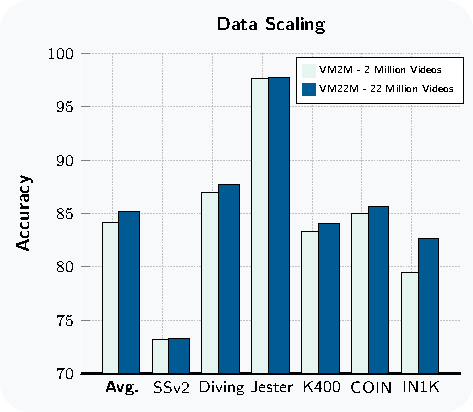
\includegraphics[width=\linewidth]{assets/vm2m_vs_vm22m.pdf}
    \end{subfigure}\hspace{3em}
    \begin{subfigure}[b]{0.35\textwidth}
        \centering
        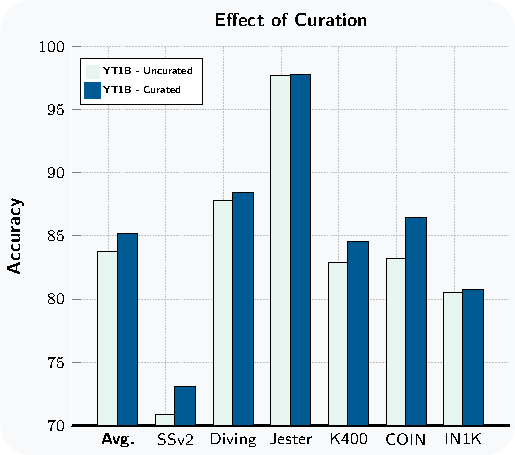
\includegraphics[width=\linewidth]{assets/curated_vs_uncurated.pdf}
    \end{subfigure}
    \caption{{\bf Data Scaling \& Curation}. We train and compare models on different data-mixes. Models are ViT-L/16 trained for 90K iterations using a cosine learning schedule following~\citet{bardes2024revisiting}. {\bf (Left)} We compare the performance of a ViT-L/16 model pretrained on the VM2M dataset and our VM22M dataset. Training on the VM22M dataset leads to a $+1$ point improvement in average performance. Performance improvement is more pronounced on appearance-based tasks such as Kinetics-400, COIN, and ImageNet {\bf (Right)} We compare the performance of a ViT-L/16 model pretrained on YT1B and a model pretrained on our Curated-YT1B dataset, which leverages our cluster-based curation. Training on the curated dataset leads to a $+1.4$ point improvement on average performances, showing the effectiveness of data-curation.}

    \label{fig:vjepa2_data_scaling}
\end{figure}

\paragraph{\bf Data Curation.}
YT1B is a large video dataset, consisting of 1.4 million video-hours, with no curation and minimal filtering compared to smaller video datasets (like Kinetics and Something-Something v2). Because uncurated and unbalanced data can hinder model performance~\citep{assran2022hidden, oquab2023dinov2}, we filter YT1B by adapting an existing retrieval-based curation pipeline to handle videos. Specifically, we  extract scenes from YT1B videos, compute an embedding vector for each scene, and then use a cluster-based retrieval process~\citep{oquab2023dinov2} to select video scenes according to a target distribution, which is composed of the Kinetics, Something-Something v2, COIN and EpicKitchen training datasets. We describe the details of the dataset construction procedure in \Cref{app:pretraining_data_appendix}. Similar to \cite{oquab2023dinov2}, we ensure that none of the videos from the target validation sets are contained in the initial, uncurated data pool.

In \Cref{fig:vjepa2_data_scaling} (Right), we compare the average performance on visual understanding evaluations between a ViT-L model pretrained on uncurated YT-1B data and a comparable model trained on our Curated-YT-1B dataset. Training with the curated dataset yields a $+1.4$ point average performance improvement over the uncurated baseline. Notably, the Curated-YT-1B-trained model achieves competitive performance relative to the full VM22M dataset at the ViT-L scale. However, larger-scale models benefit more from VM22M training (see \Cref{app:pretraining_data_appendix}), suggesting that combining Curated-YT-1B with other data sources enhances scalability.


\subsection{Pretraining Recipe}
\label{subsec:model_training}

\paragraph{\bf Scaling Model Size.}
To explore the scaling behavior of our model, we trained a family of encoder models with parameter counts ranging from 300 million (ViT-L) to 1 billion (ViT-g) parameters. All encoder architecture details are provided in \Cref{table:vit_architecture} in the appendix. Note that each encoder uses the same predictor architecture, similar to a ViT-small.
We report the average performance of these encoders on visual understanding tasks in \Cref{fig:vjepa2_scaling} (Left). Scaling the model size from 300 million (ViT-L) to 1 billion (ViT-g) parameters yields a $+1.5$ points average performance improvement. Both motion and appearance understanding tasks benefit from scaling, with SSv2 improving by $+1.6$ points and Kinetics by $+1.5$ points (cf.\Cref{tb:understanding_main}). These results confirm that self-supervised video pretraining effectively leverages larger model capacities, up to the 1B-parameter ViT-g.

\begin{figure}[!t]
    \centering
    \begin{subfigure}[b]{0.32\textwidth}
        \centering
        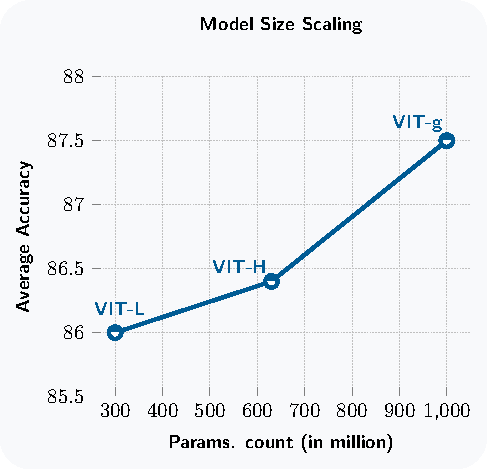
\includegraphics[width=0.96\linewidth]{assets/probe_model_scaling.pdf}
    \end{subfigure}
    \begin{subfigure}[b]{0.32\textwidth}
        \centering
        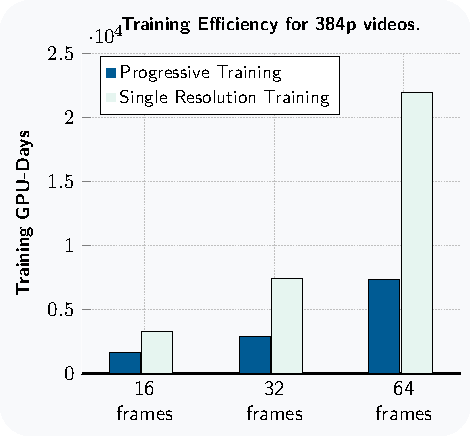
\includegraphics[width=\linewidth]{assets/annealing_compute_bars.pdf}
    \end{subfigure}
    \begin{subfigure}[b]{0.32\textwidth}
        \centering
        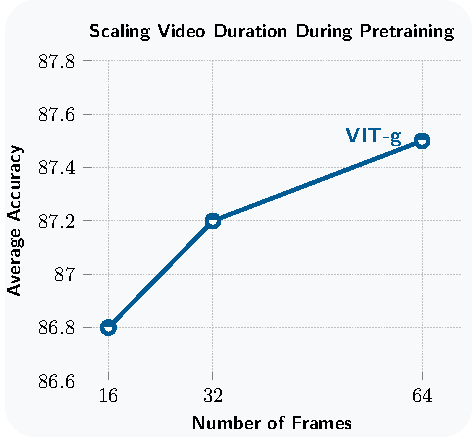
\includegraphics[width=\linewidth]{assets/anneal_frame_counts.pdf}
    \end{subfigure}
    \caption{{\bf Model Scaling.} We explore the impact of scaling model size and input video resolution. All models are trained on the VideoMix22M pretraining dataset.
{\bf (Left)} Average performance across six understanding tasks as a function of model scale. Models are trained with a constant learning rate until performance plateaus on downstream tasks. We then cool down the model using 64 frames at $256\times256$ resolution and report post-cooldown performance. Scaling the model size from 300M to 1B parameters yields a $+1.7$ point average improvement.
{\bf (Middle)} Training times (GPU-days) for ViT-g on A100 GPUs when training videos at $384\times384$ resolution with different numbers of frames per clip. We compare progressive resolution training (252K iterations at 16 frames / $256\times256$ resolution, followed by 12K cooldown iterations at $384\times384$ resolution) to the projected time for full-resolution training. Progressive training provides up to 8$\times$ speedup, significantly reducing the pretraining compute requirement.
{\bf (Right)} Effect of inscreasing video duration at cooldown on downstream performance for ViT-g. Even when only using 16-frame clips during inference/evaluation, increasing video duration during the cooldown phase of training improves average task performance by $+0.7$ points.
}
    \label{fig:vjepa2_scaling}
\end{figure}


\paragraph{\bf Training Schedule.}
\model model training employs a warmup-constant learning rate schedule followed by a cooldown phase \citep{zhai2022scaling, hagele2024scaling}. Similarly to \citet{hagele2024scaling}, we found that this schedule performs comparably to a half-cosine schedule~\citep{loshchilov2016sgdr}; it also makes exploring long training runs more cost-effective, since multiple cooldown runs can be started from different checkpoints of the constant phase.
We simplified the recipe from \citet{bardes2024revisiting} by maintaining fixed teacher EMA and weight decay coefficients instead of using ramp-up schedule, as these variations showed minimal impact on downstream understanding tasks. \Cref{fig:v1_to_v2} shows that extending the training schedule from 90K to 252K iterations yields a +0.8 average performance improvement with ViT-g models, validating the benefits of extended training durations. This schedule also facilitates progressive training by incrementally increasing video resolution during the cooldown phase.


% \newpage

\section{Conclusion}
\label{section:conclusion}

This study demonstrates how joint-embedding predictive architectures, learning in a self-supervised manner from web-scale data and a small amount of robot interaction data, can yield a world model capable of understanding, predicting, and planning in the physical world.
\model achieves state-of-art performances on action classification requiring motion understanding and human action anticipation. \model also outperforms previous vision encoders on video questions-answering tasks when aligned with a large-language model. Additionally, post-training an action-conditioned world model, \acModel, using \model's representation, enables successful zero-shot prehensile manipulation tasks, such as Pick-and-Place, with real-world robots. These findings indicate \model is a step towards developing advanced AI systems that can effectively perceive and act in their environment.

\paragraph{\bf Future work.} There are several important avenues for future work to address limitations of \model. First, in this work we have focused on tasks requiring predictions up to roughly 16 seconds into the future. This enables planning for simpler manipulation tasks, like grasp and reach-with-object, from a single goal image. However, to extend this to longer-horizon tasks such as pick-and-place or even more complex tasks, without requiring sub-goals will require further innovations in modeling. Developing approaches for hierarchical models capable of making predictions across multiple spatial and temporal scales, at different levels of abstraction, is a promising direction.

Second, as mentioned in \Cref{sec:robot_planning}, \acModel currently relies upon tasks specified as image goals. Although this may be natural for some tasks, there are other situations where language-based goal specification may be preferable. Extending the \acModel to accept language-based goals, e.g., by having a model that can embed language-based goals into the \acModel representation space, is another important direction for future work. The results described in \Cref{section:language_understanding}, aligning \model with a language model, may serve as a starting point.

Finally, in this work we scaled \model models up to a modest 1B parameters. The results in \Cref{section:stage1} demonstrated consistent performance improvements while scaling to this level. Previous work has investigated scaling vision encoders to as large as 20B parameters~\citep{zhai2022scaling,carreira2024scaling}. Additional work is needed in this direction to develop scalable pre-training recipes that lead to sustained performance improvements with scale.

\section*{Acknowledgements}

We thank
Rob Fergus, Joelle Pineau, Stephane Kasriel, Naila Murray, Mrinal Kalakrishnan, Jitendra Malik,
Randall Balestriero, Julen Urain,
Gabriel Synnaeve, Michel Meyer, Pascale Fung, Justine Kao, Florian Bordes, Aaron Foss,
Nikhil Gupta, Cody Ohlsen, Kalyan Saladi, Ananya Saxena, Mack Ward, Parth Malani, Shubho Sengupta, Leo Huang,
Kamila Benzina, Rachel Kim,
Ana Paula Kirschner Mofarrej, Alyssa Newcomb, Nisha Deo, Yael Yungster, Kenny Lehmann, Karla Martucci,
and the PerceptionLM team, including Christoph Feichtenhofer, Andrea Madotto, Tushar Nagarajan, and Piotr Dollar
for their feedback and support of this project.



\clearpage
\newpage
\bibliographystyle{kling/plainnat}
\bibliography{paper}

\clearpage
\newpage
\beginappendix


\section{\model Pretraining}
\label{app:vjepa2_pretraining}


\subsection{Pretraining Hyperparameters}
As detailed in \Cref{subsec:model_training}, our training pipeline consisted of two phases: 1) a constant learning rate phase and 2) a cooldown phase.
For all models, we trained in the first phase until we observed plateauing or diminishing performance on the IN1K, COIN, and SSv2 tasks. At this point, we initiated the cooldown phase.
\begin{table}[h]
    \small
    \caption{\small{\bf Pretraining Hyperparameters.} Common parameters for pretraining large computer vision models. We report these parameters for both the primary training phase and the cooldown phase.}
    \centering
    \label{tab:pretraining_params}
    \begin{tabular}{l c c}
      \bf Parameter & \bf Primary Phase & \bf Cooldown Phase \\
        \toprule
        Number of frames & 16 & 64 \\
        Frames per Second & 4.0 & 4.0 \\
        Crop Size & 256 & [256, 384, 512] \\
        Random Resize Aspect Ratio & [0.75 1.35] & [0.75, 1.35] \\
        Random Resize Scale & [0.3, 1.0] & [0.3, 1.0] \\
        Steps & Variable & 12000 \\
        Warmup Steps & 12000 & N/A \\
        Batch Size (global) & 3072 & 3072 \\
        Starting Learning Rate & 1e-4 & 5.25e-4 \\
        Final Learning Rate & 5.25e-4 & 1e-6  \\
        Weight Decay & 0.04 & 0.04 \\
        EMA & 0.99925 & 0.99925 \\
        Spatial Mask Scale & [0.15, 0.7] & [0.15, 0.7] \\
        Temporal Mask Scale & [1.0, 1.0] & [1.0, 1.0] \\
        Mask Aspect Ratio & [0.75 1.5] & [0.75, 1.5] \\
        Tubelet Size & 2 & 2 \\
        Patch Size & 16 & 16 \\
        \bottomrule
    \end{tabular}
\end{table}

Training in the first phase began with a learning rate warmup for 12,000 steps followed by a constant learning rate for the rest of the phase.
We checked evaluations every 60,000 steps.
The cooldown phase began with a learning rate at 5.25e-4, which was linearly ramped down to the final learning rate.
Throughout both phases, all other hyperparameters were kept constant.

In the cooldown phase we increased the number of frames per clip while keeping the frames-per-second constant, as we saw a substantial benefit from feeding the model more frames (see \Cref{fig:vjepa2_scaling}).
In addition, we also increased the crop size of the model in this phase, which gave a substantial benefit to tasks like IN1K, which goes from 84.6 at a 256 crop to 85.1 at a 384 crop.
Hyperparameters for both phases are summarized in \Cref{tab:pretraining_params}.

\begin{table}[h]
    \small
    \caption{\small{\bf Abbreviated Pretraining Hyperparameters.} Common parameters for pretraining large computer vision models, targeting our abbreviated recipe.}
    \centering
    \label{tab:abbreviated_pretraining_params}
    \begin{tabular}{l c}
      \bf Parameter & \bf Abbreviated Recipe \\
        \toprule
        Number of frames & 16 \\
        Frames per Second & 4.0 \\
        Crop Size & 256 \\
        Random Resize Aspect Ratio & [0.75 1.35] \\
        Random Resize Scale & [0.3, 1.0] \\
        Steps & 90000 \\
        Warmup Steps & 12000 \\
        Batch Size (global) & 3072 \\
        Starting Learning Rate & 2e-4 \\
        Larning Rate & 6.25e-4 \\
        Final Learning Rate & 1e-6 \\
        Starting Weight Decay & 0.04 \\
        Final Weight Decay & 0.4 \\
        Starting EMA & 0.999 \\
        Final EMA & 1.0 \\
        Spatial Mask Scale & [0.15, 0.7] \\
        Temporal Mask Scale & [1.0, 1.0] \\
        Mask Aspect Ratio & [0.75 1.5] \\
        Tubelet Size & 2 \\
        Patch Size & 16 \\
        \bottomrule
    \end{tabular}
\end{table}
Throughout the Appendix, we refer to a ``abbreviated'' training recipe that corresponds to a 90,000-step training following the procedure of~\citet{bardes2024revisiting}.
There are a few key differences with the abbreviated recipe.
The first is the learning rate: the abbreviated recipe begins with a linear warmup followed by a cosine decay.
The second are the schedules for weight decay and EMA, which are linearly ramped from a starting to a final value.
The last is the total number of steps, which is restricted to 90,000.
We use the abbreviated schedule for several of our ablations on data mixtures, as this allows us to interrogate the effects of data curation on a shorter compute budget.

\subsection{Pretraining data}
\label{app:pretraining_data_appendix}

We began curation of YT1B by applying scene extraction via the PySceneDetect library,\footnote{\url{https://github.com/Breakthrough/PySceneDetect}} which splits videos into clips at scene transitions.
We discard scenes shorter than 4 seconds, retaining 316 million scenes.
The DINOv2 ViT-L model is then applied on the middle frame of each clip to extract scene embeddings.
YT1B embeddings are then clustered into 1.5 million clusters, using the same clustering strategy as~\citet{oquab2023dinov2}.
Embeddings are also extracted in the same manner for all videos in the target distribution, then assigned to the closest YT1B cluster.
We only keep those clusters to which at least one target video was assigned---about 210k clusters out of the original 1.5 million. The retained clusters contain 115 million scenes.

Cluster-based retrieval matches the support, but not the weighting, of the target distribution.
We use a weighted sampling scheme to rebalance the data to better match the target distribution.
W sample from the clusters using a weighted sampling strategy: $w_c = \sum_{d=1}^{D} w_d \times \frac{N_{d,c}}{N_d}$
where $w_c$ is the weighting coefficient for the $c$th cluster, $w_d$ is the weighting coefficient for the $d$th target dataset (from \Cref{table:retrieval_stats}, $N_{d,c}$ is the number of samples from the $d$th dataset in the $c$th cluster, $N_d$ is the total number of samples in the $d$th dataset, and $D$ is the total count of target datasets.
We assigned the retrieval weights approximately based on how many scenes were retrieved by each target dataset, with some extra weighting assigned to EpicKitchen.
This gave a final curated dataset with statistics more closely matching those of handcrafted datasets from the literature.
We found that in isolation, using curated YT1B in place of its uncurated counterpart gave much better results on downstream  understanding tasks (see \Cref{fig:vjepa2_data_scaling}).


\begin{table}[h]
    \centering
    \small
    \caption{
      \textbf{Data Curation Statistics.} We summarized the number of extracted scenes and hours of videos across clusters extracted from YT1B. The final line includes duplicates among retrievals of K710, SSv2, COIN, and EpicKitchen.}
    \begin{tabular}{ccccccc}
    \toprule
    Retrieval Target & Cluster Count & Number of Scenes & Retrieval Weight  \\
    \midrule
    Uncurated YT1B & 1.5M & 316M  \\
    \midrule
    K710 & 170k & 100M &  0.7 \\
    SSv2 & 41k & 19M &  0.125 \\
    COIN & 37k & 21M &  0.125 \\
    EpicKitchen & 4k &  13k & 0.05 \\
    \midrule
    Final Curated (includes duplicates) & 210k & 115M
    \end{tabular}
    \label{table:retrieval_stats}
\end{table}
The overall statistics from how many clusters and scenes were retrieved with this strategy are summarized in \Cref{table:retrieval_stats}.
The overall dataset is weighted towards clusters retrieved with K710. This, combined with its retrieval weight of 0.7, gives the overall curated dataset a heavy Kinetics weighting that we saw reflected in K400 performance for our ablation experiments (see \Cref{app:data_curation_app_additional_results}).
As shown in \Cref{table:pretraining_dataset} in the main body, we combined this Curated YT1B with SSv2, Kinetics, HowTo100M, and ImageNet to create our final VM22M dataset.

\end{document}


